% $Header: /cvsroot/latex-beamer/latex-beamer/solutions/generic-talks/generic-ornate-15min-45min.en.tex,v 1.4 2004/10/07 20:53:08 tantau Exp $

%\documentclass[compress]{beamer}
\documentclass{beamer}
%\colorlet{structure}{magenta}

%\usepackage{paralist}
%\usecolortheme[named=yellow]{structure}


\mode<presentation>
{

  %\usetheme{Warsaw}
  %\usetheme{AnnArbor}
  %\usetheme{Boadilla}
  \usetheme{CambridgeUS}
  %\usetheme{Madrid}
  % or ...

  \setbeamercovered{transparent}
  % or whatever (possibly just delete it)
}


\usepackage[english]{babel}
% or whatever

\usepackage[latin1]{inputenc}
% or whatever

\usepackage{times}
\usepackage[T1]{fontenc}

% Or whatever. Note that the encoding and the font should match. If T1
% does not look nice, try deleting the line with the fontenc.

\title[uComp Prot\'eg\'e Plugin]{The uComp Prot\'eg\'e Plugin:\\ Crowdsourcing Enabled Ontology Engineering}


%\subtitle{WebS '09} % (optional)

\author[Hanika et al.]{
\small{
Florian Hanika \inst{1} \texttt{florian.hanika@wu.ac.at} \\
\textbf{Gerhard Wohlgenannt} \inst{1} \texttt{wohlg@ai.wu.ac.at} \\
Marta Sabou\inst{2}  \texttt{marta.sabou@ifs.tuwien.ac.at} \\
}}

\institute{Institut f. Informationswirtschaft}

% - Use the \inst{?} command only if the authors have different
%   affiliation.

\institute[InfoBiz, WU Vienna] % (optional, but mostly needed)
{
  \inst{1}%
  %Project RAVEN/Adonis,
  Institute f. Information Business,
  \textbf{Vienna Univ. of Economics (WU)}, Austria

  \inst{2}%
  %Project RAVEN/Adonis,
  \textbf{Technical University (TU), Vienna}, Austria
}

\date[EKAW 2014]{EKAW 2014\\ \today}

\subject{Talks}
% This is only inserted into the PDF information catalog. Can be left
% out. 


% If you have a file called "university-logo-filename.xxx", where xxx
% is a graphic format that can be processed by latex or pdflatex,
% resp., then you can add a logo as follows:

% \pgfdeclareimage[height=0.5cm]{university-logo}{university-logo-filename}
% \logo{\pgfuseimage{university-logo}}



% Delete this, if you do not want the table of contents to pop up at
% the beginning of each subsection:
%\AtBeginSubsection[]
%{
%  \begin{frame}<beamer>
%    \frametitle{Outline}
%    %\tableofcontents[currentsection,currentsubsection]
%    \tableofcontents[currentsection]
%  \end{frame}
%}

%\AtBeginSection[]
% {
%   \begin{frame}<beamer>
%     \frametitle{Outline}
%     %\tableofcontents[currentsection,currentsubsection]
%     %\tableofcontents[currentsection]
%   \end{frame}
% }
% 


% If you wish to uncover everything in a step-wise fashion, uncomment
% the following command: 

% \beamerdefaultoverlayspecification{<+->}


\begin{document}
%\setbeamertemplate{footline}[page number]

\begin{frame}
  \titlepage
\end{frame}

%\begin{frame}
%  \frametitle{REMOVE ME}
%  \begin{itemize}
%  \item Length: 20min sharp .. 22.5min for person incl discussion! 
%  \item GOAL: 15-20 slides (dep on content on slides) \\
%
%
%* given an overview over the ontology learning framework
%
%* present the 2 matrices ... (evidence confidence matrix + source impact vector)
%
%* Future work:
%    implementation -- ongoing :-)
%        open point:
%            what is a good method to feed back information from gwaps (eg. tagged concepts)
%            into the spreading activation net --
%            ie how to optimize the weights (the source impact vector)
%
%            not an expert in these techniques -- feedback very welcome
%
%  \end{itemize}
%\end{frame}



% TODO -- remove section bar

\section{Introduction}
%\subsection{The uComp Prot\'eg\'e Plugin}
\begin{frame}
  \frametitle{Introduction - What is this about?}
  \begin{itemize}
        \item The \textbf{integration} of \structure{crowdsourcing} into the \structure{ontology engineering workflow} with the help of a \structure{Prot\'eg\'e plugin}.
    \vspace{0.5cm}
        \item Certain tasks like \structure{validating} concept relevance, subClassOf relations, etc.~are outsourced to crowd workers.
    \vspace{0.5cm}
        \item Evaluate the impact on \structure{quality, cost and time} of using crowdsourcing instead of domain experts.
  \end{itemize}
\end{frame}

\begin{frame}
  \frametitle{Research Questions}
  \begin{itemize}
        \item \structure{Which tasks} can be crowdsourced? ($\rightarrow{}$ literature review)
    \vspace{0.5cm}
        \item How to \structure{support} crowdsourcing enabled ontology engineering? ($\rightarrow{}$ build a tool) 
    \vspace{0.5cm}
        \item Is crowd-based ontology engineering \structure{effective and scalable}? ($\rightarrow{}$ evaluation) 
  \end{itemize}
\end{frame}


\section{Human Computation}
\begin{frame}
  \frametitle{Human Computation (HC)}
  \begin{itemize}
        \item \dots using \structure{human input} for tasks/problems that computers cannot solve (yet)
    \vspace{0.5cm}
        \item \structure{Different types:} \textbf{Games with a Purpose, paid crowdsourcing}, and altruism. 
    \vspace{0.5cm}
        \item Typical (mechanised labour): paid crowdsourcing to solve \structure{micro-tasks}, such as: \\
    \vspace{0.1cm}
        \texttt{Is every \textbf{dog} a \textbf{mammal}?} % TODO .. make prettier
  \end{itemize}
\end{frame}

\begin{frame}
  \frametitle{Related Work / Existing Efforts}
    Crowdsourcing already \textbf{widely used} in different areas, for example in 
    \vspace{0.2cm}
  \begin{itemize}
    \item \textbf{NLP community:} GATE Crowdsourcing Plugin [Bontcheva et al, 2014], 
    \item ZenCrowd (entity linking), CrowdMap (ontology alignment)
    \item Validation of subClassOf relations [Noy et al., 2013]
  \end{itemize}
\end{frame}

\begin{frame}
  \frametitle{Why use HC in Ontology Construction / Engineering?}
  \begin{enumerate}
    \item \structure{Ontology creation} typically needs domain experts and is \textbf{expensive and cumbersome}
    \item \structure{Ontology learning} often used to \textbf{bootstrap} the ontology building process 
    \item Using the \structure{crowd} is feasible to further \textbf{reduce cost and effort}
    \item It has been demonstrated that \structure{crowd-workers provide high-quality assessments}, especially for general knowledge domains [Noy et al., 2013] %TODO: maybe add others
    \item Crowdsourcing has been proven useful, but \structure{high investments} necessary for setting up infrastructure and task $\rightarrow{}$ \textbf{tool support} needed, eg. from inside Prot\'eg\'e
  \end{enumerate}
\end{frame}


\section{The Crowdsourcing Workflow}

\begin{frame}
  \frametitle{Typical Ontology Engineering (OE) Tasks in Literature}
    \huge Step 1: which OE tasks? \\ \large
    \vspace{0.5cm}
    \dots where crowdsourcing has been applied or appears feasible
    \vspace{0.2cm}
  \begin{itemize}
    \item Specification of \textbf{Term Relatedness}: are two terms related?
    \item Verification of \textbf{Relation Correctness}
    \item Specification of \textbf{Relation Type}
    \item Verification of \textbf{Domain Relevance}
  \end{itemize}
\end{frame}


\begin{frame}
  \frametitle{The Workflow of the Plugin}
  \framesubtitle{Figure: Main Stages when using the uComp Plugin}
   \center
  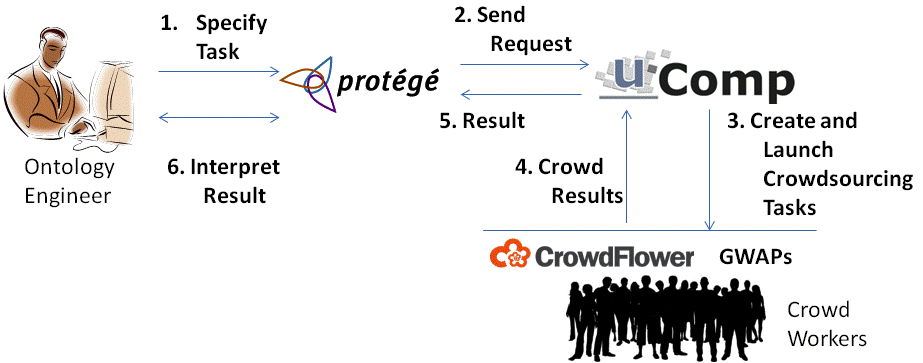
\includegraphics[height=1.9in]{images/process}
\end{frame}

% TODO fill slide
\begin{frame}
  \frametitle{The uComp API}
  \begin{itemize}
        \item REST API 
        \item \structure{Communication} between the Prot\'eg\'e plugin and the crowdsourcing platforms

        \item \structure{\textbf{configuration file}}
          \begin{itemize}
                \item \textbf{API key:} can be obtained from us
                \item \textbf{Number of judgements} per unit 
                \item \$-cents paid per judgement 
          \end{itemize}

  \end{itemize}
\end{frame}



\section{The Prot\'eg\'e Plugin}

\begin{frame}
  \frametitle{The Prot\'eg\'e Plugin}
    \huge Step 2: Tool Support \\ \large
    \vspace{0.5cm}
 
  \begin{itemize}
        \item Plugins usually done as \textbf{views} in Prot\'eg\'e
    \vspace{0.5cm}
        %\item We identified typical OE crowdsourcing tasks from literature and built plugin support for them
    \vspace{0.5cm}
        \item \structure{Accessible for download} from inside Prot\'eg\'e (via plugin repository) -- named \structure{uComp Crowdsourcing Validation plugin}
  \end{itemize}
\end{frame}


\begin{frame}
  \frametitle{Domain Relevance Verification}
  \framesubtitle{The user interface}
   \center
  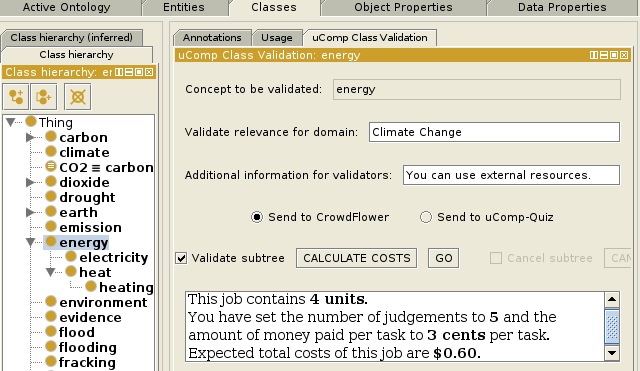
\includegraphics[height=2.5in]{images/cc_class_new}
\end{frame}

\begin{frame}
  \frametitle{Typical Elements of the UI}
  \begin{itemize}
        \item \structure{Task-specific information:} eg. concept to be verified 
        \item \structure{Generic Information:} ontology domain, etc. (pre-filled)
        \item \structure{Task description:} Predefined descriptions (for CF users) can be extended here
        \item \structure{Recursive control:} also verify all subconcepts?
        \item CrowdFlower or GWAP? 
        \item Calculate cost 
  \end{itemize}
\end{frame}

\begin{frame}
  \frametitle{The Workflow}
  \framesubtitle{Figure: Main stages when using the uComp plugin}
   \center
  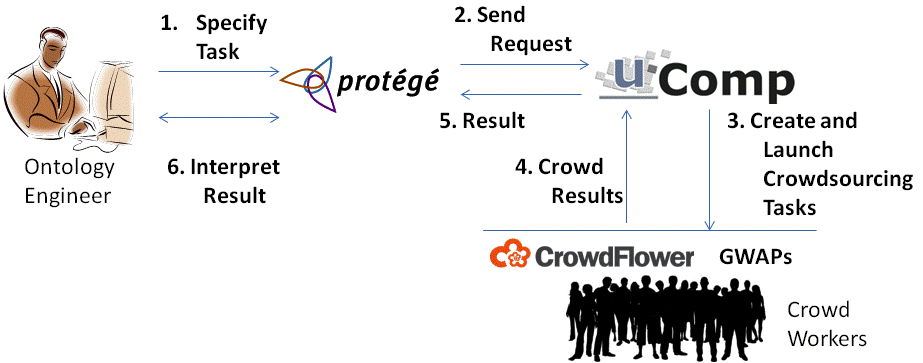
\includegraphics[height=1.9in]{images/process}
\end{frame}


\begin{frame}
  \frametitle{subClassOf Relation Validation}
  %\framesubtitle{}
   \center
  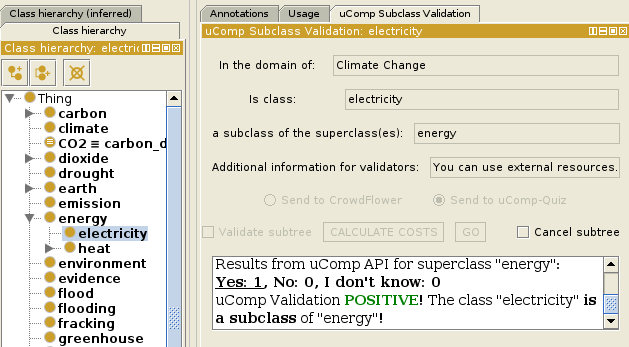
\includegraphics[height=2.5in]{images/subclass_val_new}
\end{frame}


\begin{frame}
  \frametitle{Generated CrowdFlower Job Interface}
  \framesubtitle{subClassOf Task}
   \center
  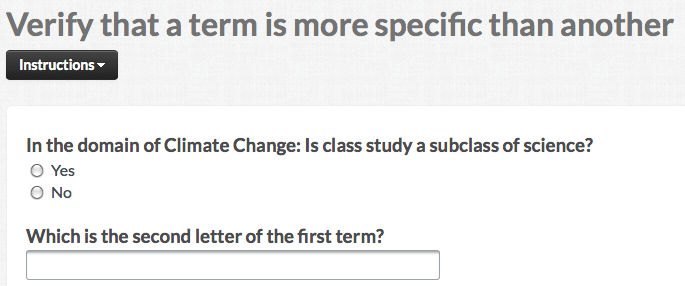
\includegraphics[height=1.9in]{images/CFsubclasscheck}
\end{frame}


\begin{frame}
  \frametitle{InstanceOf Relation Validation}
  %\framesubtitle{}
   \center
  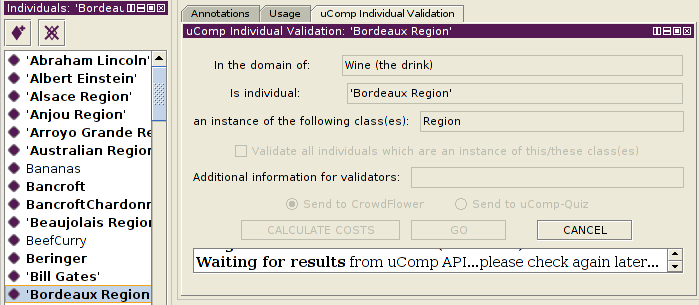
\includegraphics[height=2.1in]{images/screenshot_indiv}
\end{frame}

% TODO .. add other tasks --> add images -- but just skip over them
%\begin{frame}
%  \frametitle{Domain/Range Restrictions Validation}
%  %\framesubtitle{}
%   \center
%  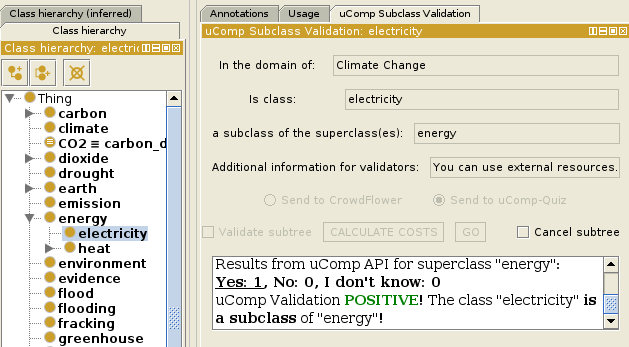
\includegraphics[height=2.5in]{images/subclass_val_new}
%\end{frame}

%\begin{frame}
%  \frametitle{Valdiation Tasks Supported}
%  \begin{itemize}
%        \item Concept relevance 
%        \item SubClassOf relations
%        \item InstanceOf relations 
%        \item Domain and Range restrictions 
%        %\item Suggesting relation types for unlabelled relations
%  \end{itemize}
%\end{frame}


% empty slide :-)
%\begin{frame}
%  \frametitle{}
%  \begin{itemize}
%        \item 
%    \vspace{0.5cm}
%        \item 
%    \vspace{0.5cm}
%        \item
%  \end{itemize}
%\end{frame}


\section{Evaluation}

% TODO fill
\begin{frame}
 \frametitle{Setup of Feasibility Evaluation}

    \huge Step 3: Evaluation \\ \large
    \vspace{0.5cm}
    \large
    First: \structure{Feasibility}
 
  \begin{itemize}
        \item \textbf{Domains}: Climate change and finance
        \item \textbf{Ontology size}: ca 100 concepts, ca 40 subClassOf relations per ontology
        \item \textbf{Evaluators}: 8 domain experts (Manual setting), 4 experts using CrowdFlower (Crowd setting) instead
  \end{itemize}
\end{frame}

\begin{frame}
  \frametitle{Evaluation Tasks}
  \begin{itemize}
        \item \textbf{Domain relevance}: For each \structure{concept} decide if it is \structure{relevant for the domain}
        \item \textbf{Subsumption}: For each \structure{subClassOf relation} -- verify if it is correct.
        \item InstanceOf relations
        %\item \textbf{Relation Suggestion}: from ontology learning, no gold standard (baseline), using agreement as measure of quality 
  \end{itemize}
\end{frame}


\begin{frame}
  \frametitle{Results -- Feasibility -- Time and Cost}
        \begin{table}
        \small
        \center
        \begin{tabular}{|c|c|c|} \hline
            & \multicolumn{2}{|c|}{\textbf{Climate Change}} \\ 
           % \cline{2-5}
                & \multicolumn{2}{|c|}{\textbf{Ontology}} \\ 
                  \cline{2-3}
                & \textbf{Domain Rel} & \textbf{SubClass Validation} \\ \hline

        \textbf{Time Manual}         & 27.4    & 23.0  \\ \hline
        \textbf{Time Crowd}          & 242     & 282   \\ \hline
        \textbf{Time Saved}          & 0.11    & 0.08  \\ \hline
 
        \textbf{Cost Manual}         &  11.9   & 9.9   \\ \hline
        %\textbf{Cost Crowd}          &  9.4    & 4.5   \\ \hline %% 5 votes a $0.05
        %\textbf{Cost Crowd Cheap}    &  2.1    & 1.33  \\ \hline %% 3 votes a $0.01
        %\textbf{Cost Saved Cheap}    &  83\%   & 86\%  \\ \hline
        \textbf{Cost Crowd}          &  2.1    & 1.33  \\ \hline %% 3 votes a $0.01
        \textbf{Cost Saved}     &  83\%   & 86\%  \\ \hline
         \end{tabular}
        \caption{Task duration in minutes and costs (in \$)}


    \label{table:eval_qual}
\end{table}

\end{frame}


\begin{frame}
  \frametitle{Results -- Feasibility -- Agreement}

        \begin{table}
        \small
        \center
        \begin{tabular}{|c|c|c|} \hline
            & \multicolumn{2}{|c|}{\textbf{Climate Change}} \\ 
           % \cline{2-5}
                & \multicolumn{2}{|c|}{\textbf{Ontology}} \\ 

                  \cline{2-3}
                                              & \textbf{Concept Relevance} & \textbf{Subclass Val.} \\ \hline
        %\textbf{Setting 1 - Percentage valid} & 0.65          & 0.5          \\ \hline
        \textbf{Manual}                   & 0.338 (8)     & 0.502 (8)      \\ \hline
        \textbf{Crowd}                    & 0.633 (4)     & 0.841 (4)      \\ \hline
        \textbf{ManualCrowd}              & 0.392 (12)    & 0.582 (12)     \\ \hline
        \end{tabular}
        \caption{Fleiss' Kappa values of \structure{inter-rater agreement} per setting and when combining the data of the two settings.}
    \label{table:eval_qual}

\end{table}
\vspace{0.5cm}
\small \textbf{Interpretation:} The agreement between the crowd and experts is higher than among experts, possibly because crowdsourcing data is the \structure{majority view}.
\end{frame}


%\begin{frame}
%  \frametitle{Results -- Scalabily}
%        \begin{table}
%        \footnotesize
%        \center
%        \begin{tabular}{|c|c|c|c|c|} \hline
%            & \multicolumn{2}{|c|}{\textbf{Climate Change}} & \multicolumn{2}{c|}{\textbf{Finance}}  \\
%           % \cline{2-5}
%                & \multicolumn{2}{|c|}{\textbf{Ontology}} & \multicolumn{2}{c|}{\textbf{Ontology}}  \\
%
%                  \cline{2-5}
%                                              & \textbf{T\_DomRel} & \textbf{T\_SubsCorr} & \textbf{T\_DomRel} & \textbf{T\_SubsCorr} \\ \hline
%        %\textbf{Setting 1 - Percentage valid} & 0.65          & 0.5             & 0.69            & 0.15            \\ \hline
%        \textbf{S\_Manual}                   & 0.338 (8)     & 0.502 (8)       & 0.496 (8)       & 0.419 (8)       \\ \hline
%        \textbf{S\_Crowd}                    & 0.633 (4)     & 0.841 (4)       & 0.520 (4)       & 0.826 (4)       \\ \hline
%        \textbf{S\_ManualCrowd}              & 0.392 (12)    & 0.582 (12)      & 0.505 (12)      & 0.508 (12)      \\ \hline
%        \end{tabular}
%        \caption{Fleiss' Kappa values of inter-rater agreement per setting and when combining the data of the two settings.}
%
%    \label{table:eval_qual}
%\end{table}
%\end{frame}


% TODO fill
\begin{frame}
  \frametitle{Setup of Scalability Evaluation}
  \begin{itemize}
        \item Done for \structure{SWJ extended version} of the paper
    \vspace{0.1cm}
        \item Assess the plugin's effect on the time, cost and quality for \structure{large, real-life and domain specific ontologies}
    \vspace{0.2cm}
        \item \textbf{Domain}: \structure{anatomy (medical)} -- human.owl ontology which represents the human anatomy part of the NCI thesaurus (from Anatomy track of the Ontology Matching Initiative 10)
        \item \textbf{Ontology size}: \structure{4304 concepts, 3761 subClassOf relations}
        \item \textbf{Evaluators}: \structure{time and cost estimations} for experts, based on wage of a research scientist of \$26 per hour
        \item \textbf{Ontology}: we assume it is correct, can use it as a baseline
  \end{itemize}
\end{frame}

\begin{frame}
\frametitle{Introducing Errors}
  \begin{itemize}
        \item \textbf{Domain relevance check}: we randomly added \textbf{1000} concepts from the domains of \structure{tennis} and \structure{climate change}
        \item \textbf{Subsumption validation}: we randomly selected 800 leaf pairs of concepts, and swapped them $\rightarrow{}$ introduce \structure{1600 wrong subClassOf relations}
  \end{itemize}
\end{frame}



\begin{frame}
  \frametitle{Results -- Scalability}
\begin{table}
\small
\center
\begin{tabular}{|l|c|c|c|c|} \hline
    & \multicolumn{2}{|c|}{\textbf{Concept relevance}} & \multicolumn{2}{c|}{\textbf{Subsumption}}  \\
        & \multicolumn{2}{|c|}{\textbf{Verification}} & \multicolumn{2}{c|}{\textbf{Verification}}  \\

          \cline{2-5}
                                      & \textbf{Crowd} & \textbf{Est. Manual} & \textbf{Crowd} & \textbf{Est. Manual} \\ \hline
\textbf{Time (Hours/Days)}                &  19/0.8   &   19.65/2.5  &  136/5.6    &  39.20 (4.9)  \\ \hline
\textbf{Cost (\$)}                   &   104+26TF  & 511     &  155+39TF   &  1019    \\ \hline
\textbf{Cost (Percentage)}           &   25\% & 100\%     &  19\%   &  100\%    \\ \hline
\textbf{Quality (Accuracy)}          & 0.99 &  --   &  0.895   &  --     \\ \hline

\end{tabular}
\caption{Results of the large scale evaluation for the two tasks. Values of the manual approach are estimated based on the results of the feasibility experiments. }
\label{table:eval_scale}
\end{table}

\end{frame}


\begin{frame}
  \frametitle{Summary of Evaluation / Interpretation}
  \begin{itemize}
        \item \textbf{Feasibility study}:
            \begin{itemize}
                \item \textbf{Cost:} reduction of 40\% to 83\% depending on settings used 
                \item \textbf{Quality:} Comparable with that of tasks performed by ontology engineers 
            \end{itemize}
\vspace{0.5cm}
        \item \textbf{Large scale / medical domain}:
            \begin{itemize}
                \item good quality results (accuracy of 89\% and 99\%)
                \item \textbf{Completion Time}: similar to domain experts 
                \item \textbf{Cost reduction}: of 75\% to 81\% 
            \end{itemize}
  \end{itemize}
\end{frame}

\begin{frame}
  \frametitle{Quality Control in Crowdsourcing (CrowdFlower)}
  \begin{itemize}
        \item Provide \structure{Gold units} -- easy questions with predefined answers to filter spammers and bots 
        \item \structure{Geographical selection:} Eg restrict workers to UK, US, AUS, \dots 
        \item \structure{Pay} reasonably -- if feeling screwed, crowdworkers will rush through units
        \item Only accept high-quality (Level 3) CrowdFlower contributors
  \end{itemize}
\end{frame}




% \subsection{Run-time}
% \begin{frame}
%  \frametitle{Evaluation -- Run-time-performance}
% \begin{table}[htb]
%   \centering
%   \begin{tabular}{|lcc|ccc|}
%    \hline
%    Run       &  concepts    & conns.        &  SPREADING    & EIGENV   & BRUTE     \\\hline
%    %Avg s-1   &  2495        & 3303          & 00:00:10 (1)  & 00:05:56 & 00:00:11  \\
%    Avg s-2   &  3843        & 9054          & 00:40:56 (91) & 00:30:05 & 00:00:57  \\
%    Avg s-3   &  6101        & 18655         & 00:38:47 (86) & 01:22:40 & 00:01:54  \\ \hline
%    Biggest   &  6842        & 22342         & 00:44:35 (109)& 01:43:46 & 00:02:35  \\
%    W/ DR     &  6842        & 22342         &    --         & 00:35:33 & --        \\ \hline
%   \end{tabular}
%   \caption{\label{eval:runtime}Run-times depending on the number of \texttt{concepts} and the number of \texttt{connections}}
% \end{table}
%
%\end{frame}

\section{Conclusions}
% TODO fill
\begin{frame}
  \frametitle{Conclusions/Contributions}

\structure{Summary:} Presented the uComp Prot\'eg\'e plugin and its evaluation
\vspace{0.7cm}

\structure{Contributions:}
    \begin{enumerate}
       \item Identified ontology engineering tasks suited for crowdsourcing 
       \item Implemented a Prot\'eg\'e plugin 
       \item Evaluations show significant cost reduction through crowdsourcing while providing acceptable quality
    \end{enumerate}
\end{frame}



\begin{frame}
  \frametitle{Future Work}

\structure{\textbf{Future work:}} \\
    \begin{enumerate}
       \item A clearer \structure{methodology} and guidelines of where crowdsourcing is helpful and where not.
       \item Towards \structure{expert sourcing:} Investigate engaging the community in a similar fashion. 
       \item \structure{Plugin development:} new tasks, improved task monitoring, etc. 
       \item Further scenarios (like ontology matching), extended usability studies.
    \end{enumerate}
\end{frame}


%------------------------------------------------------------------------------------ %

\begin{frame}
  \frametitle{Thank you!}
  %\framesubtitle{}
   \center
  
\includegraphics[height=2.7in]{images/questions}
\end{frame}


% \begin{frame}
%   \frametitle{Thank you}
%     \begin{itemize}
%      \item Questions? 
%      \item I am thankful for remarks! :-)
%     \end{itemize}
% \end{frame}



\begin{frame}
  \frametitle{Results -- InstanceOf Verification}
    \begin{table}
    \small
    \center
    \begin{tabular}{|l|c|c|c|c|} \hline
    \textbf{}            &\textbf{No. instances}& \textbf{Accuracy} & \textbf{Avg. time (Min)}&\textbf{Avg. Cost (\$)} \\ \hline
    \textbf{Manual}      & 116 & 1.0  & 45.6 &  19.76\\ \hline
    \textbf{CrowdFl.} & 116 & 1.0  & 120 & 6.31 \\ \hline

    \end{tabular}
    \caption{Results of the InstanceOf Verification (T2) task.}
    \label{table:resInstanceOf}
    \end{table}
\end{frame}


\begin{frame}
  \frametitle{Results -- Relation Type Suggestion}
    \begin{table}
    \center
    \begin{tabular}{|c|c|c|} \hline
                                           & \textbf{Climate Change} & \textbf{Tennis}  \\ \hline
      \textbf{S\_Manual}                   & 0.536 (5)               & 0.366 (5)        \\ \hline
      \textbf{S\_ManualCrowd}              & 0.531 (6)               & 0.368 (6)        \\ \hline
    \end{tabular}
    \caption{Fleiss' Kappa values of inter-rater agreement for the Specification of Relation Type (T3) task, for two domains.}
    \label{table:eval_rel_sugg}
    \end{table}

\end{frame}



\end{document}
